\chapter{Mineria de Datos \& Deep Learning }\label{cap:deep_learning}

\section{Consideraciones Iniciales}

Los rápidos avances en las tecnologías de recolección y de almacenamiento permitieron el almacenamiento de grandes cantidades de datos. Sin embargo, se probó que extraer conocimiento puede ser extremadamente difícil. En este contexto, la minería de datos combina métodos tradicionales de análisis de datos con algoritmos sofisticados para el procesamiento de grandes volúmenes de datos \cite{Tan:2005:IDM:1095618}.

La Minería de Datos (\textit{Data Mining}) es un área de investigación dentro en un contexto más amplio llamado Descubrimiento del Conocimiento en Bases de Datos (\textit{KDD – Knowledge Discovery in Databases}), cuyo objetivo principal es extraer de un conjunto de datos, el conocimiento a ser utilizado en procesos decisorios. Más específicamente, los principales objetivos de los métodos de minería de datos son una descripción de un conjunto de datos y una predicción de valores futuros de interés basado en conocimiento previo de un banco de datos \cite{Fayyad:1996:DMK:257938.257942}.
 
 En la Sección \ref{sec:kdd-datamining} son discutidos los principales conceptos de Minería de Datos y Descubrimiento del Conocimiento en Bases de Datos (KDD). En la Sección \ref{sec:machine-learning}, es  presentado los conceptos de Aprendizaje de Máquina  (\textit{Machine Learning}) y Redes Neuronales. En la Sección \ref{sec:cnn}, se analizan los conceptos de  \acf{CNNs} así como las principales  aplicaciones y casos de éxito. La Sección \ref{sec:autoencoders}, se analiza la teoría de Auto-codificadores y en la Sección \ref{sec:consideraciones-finales} se presentan las consideraciones finales del capítulo.

\section{KDD y Mineria de Datos}\label{sec:kdd-datamining}

\textbf{Descubrimiento de Conocimiento en Base de Datos (KDD)} - es el proceso de: primero, a partir de los datos, identificar patrones válidos, nuevos, potencialmente útiles y comprensivos. Segun  \cite{Fayyad:1996:DMK:257938.257942}, este proceso está compuesto de cinco etapas: selección de los datos; pre-procesamiento y limpieza de los datos; transformación de los datos; Minería de los Datos (\textit{Data Mining}); e interpretación y validación de los resultados. La interpretación entre estas diversas etapas puede ser observada en la Figura \ref{fig:processoKDD}, siendo que las tres primeras pueden ser interpretadas como un análisis exploratorio de los datos.

\begin{figure}[htp]
\centering
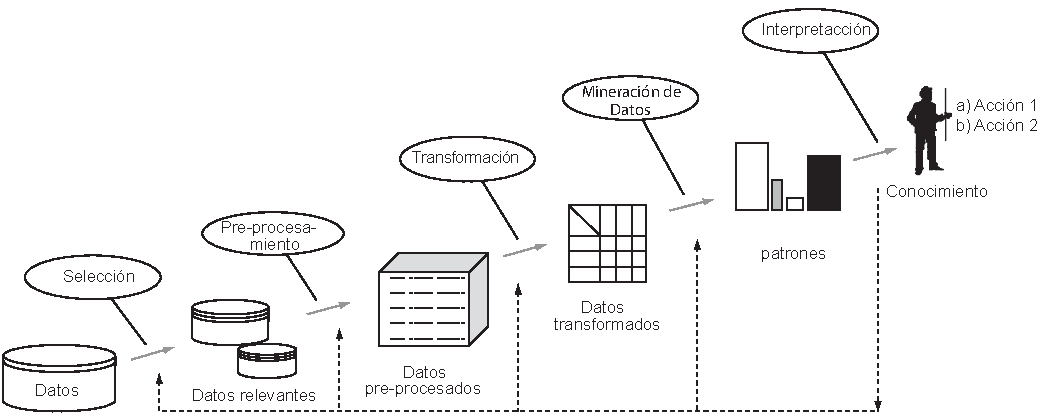
\includegraphics[width=0.99\columnwidth]{chapter3/KDD-process.pdf}
\caption{Etapas del proceso KDD. Figura adaptada de \cite{Fayyad:1996:DMK:257938.257942}.}
\label{fig:processoKDD}
\end{figure}


Los principales pasos para el proceso de KDD son:

\begin{enumerate}

    \item \textbf{Limpieza de datos:} Las bases de datos del mundo real a menudo tienen datos incompletos, con ruido e inconsistentes que pueden dañar el análisis dificultando la detección de patrones. Los procedimientos de limpieza de datos trabajan para preparar los datos para los siguientes pasos en el procesos KDD mediante el llenado de los valores que faltan, corrigiendo los datos con ruido, identificando y removiendo valores atípicos, y resolviendo inconsistencia.
    \item \textbf{Integración de datos:} En algunas circunstancias, los datos de múltiples fuentes deben fusionarse y transformadas en formas apropiadas para ser incluidas en el mismo análisis. Por lo tanto, este paso implica técnicas para integrar correctamente múltiples bases de datos, cubos de datos o archivos en un almacenamiento de datos.
    \item \textbf{Selección de datos:} Este paso corresponde a la identificación de datos relevantes para la tarea de análisis y su recuperación a partir de las bases de datos.
    \item \textbf{Transformación de datos:} En este paso, los datos son transformados o consolidados en adecuadas formas para la extracción usando operaciones, tales como el resumen, la agregación, la generalización o la normalización.
    \item \textbf{Minería de datos:} Este paso es fundamental en el proceso KDD, donde se aplican técnicas computacionales para extraer patrones desconocidos y útiles a partir de los datos.
    \item \textbf{Evaluación del patrón:} En este paso, se utilizan medidas interesantes para identificar los patrones que representan el conocimiento.

\end{enumerate}


La etapa de minería de datos incluye la definición de las tareas de minería a ser realizadas, la elección del algoritmo a ser aplicado y la extracción de patrones de interés. En la etapa siguiente, los patrones son interpretados y validados, y si los resultados no fueran satisfactorios (validos, nuevos, útiles y comprensibles), el proceso retorna a uno de los dos estados anteriores. Caso contrario, el conocimiento descubierto es consolidado \cite{Fayyad:1996:DMK:257938.257942}. El proceso KDD se refiere a todo el proceso de descubrimiento de conocimiento útil para los datos, en cuanto a la Minería de los Datos se refiere a la aplicación de algoritmos para extraer modelos de los datos.


\section{Aprendizaje de Máquina -- \textit{Machine Learning} }\label{sec:machine-learning}

    Durante las últimas décadas el aprendizaje de maquina se ha convertido en uno de los pilares de la tecnología de la información y con ello, a llegado a formar parte importante de nuestras vidas, aunque de manera imperceptible. Con la gran cantidad de datos que se generan constantemente, hay razones suficientes para creer que el análisis inteligente de datos será cada vez más generalizado como un ingrediente necesario para el progreso tecnológico, \cite{smola2008ml}.

    \subsection*{Maquinas Inteligentes}

    El cerebro es el órgano del cuerpo humano mas increíble. Este determina la forma en la que percibimos el mundo con nuestros sentidos. Desde niño el ser humanos es capas de  resolver problemas que incluso los supercomputadores más potentes no pueden resolver. Por décadas el ser humano a soñado por construir maquinas inteligentes con conciencia como la nuestra, asistentes robóticas para limpieza de nuestros hogares, autos que se manejan por si solos, microscopios que automáticamente detectan enfermedades. Pero la construcción de estas máquinas de inteligencia artificial nos obliga a resolver algunos de los problemas más complejos de la ciencia con los que hemos tenido que lidiar, comprender el funcionamiento de nuestros cerebros. \cite{dlBook}.

    \subsection*{Mecanismos del aprendizaje de maquina}

    Para hacer frente a esta clase de problemas tendremos que utilizar un tipo muy diferente de enfoque. Muchas de las cosas que aprendemos en la escuela tienen mucho en común con los programas informáticos tradicionales. Aprendemos cómo multiplicar números, resolver ecuaciones, y hacer derivadas mediante la guía de un conjunto de instrucciones. Pero las cosas que aprendemos a una edad muy temprana, las cosas que nos parecen naturales, se aprenden con el ejemplo, no por fórmulas \cite{dlBook}.
    \\\\
    Deep Learning es un subconjunto de un campo más amplio de la inteligencia artificial llamado aprendizaje de maquina o \textit{Machine Learning}, que se basa en la idea de aprender con el ejemplo. En lugar de enseñar a una computadora las reglas para resolver un problema, le damos un modelo con el que se puede evaluar ejemplos y un pequeño conjunto de instrucciones para modificar el modelo cuando se comete un error. Esperando que, con el tiempo, un modelo fuera capaz de resolver el problema con gran precisión \cite{dlBook}.
    \\\\
    Ahora formularemos esta idea matemáticamente, vamos a definir nuestro modelo como una función $h(X,\theta)$ la entrada $X$ es un ejemplo expresado en forma de vector. Por ejemplo, si $X$ fuera una imagen en escala de grises, los componentes del vector serían las intensidades de los píxeles en cada posición, como se muestra en la Figura \ref{fig:gscale}.
    \begin{figure}[htp]
        \centering
        \includegraphics[scale=0.4]{chapter3/grayscale.png}
        \caption{Vectorización de una imagen}
        \source{Fundamentals of Deep Learning, \cite{dlBook}}
        \label{fig:gscale}
    \end{figure}

    La entrada $\theta$ es un vector de parámetros que utiliza nuestro modelo, este intenta perfeccionar los valores de estos parámetros, ya que se expone a más y más ejemplos. Para comprender mejor los modelos de aprendizaje de maquina, analizaremos un ejemplo, digamos que pretendemos determinar cómo predecir el rendimiento en un examen, basándonos en el número de horas de sueño y el número de horas de estudio del día anterior. Recolectamos muchos datos y para cada punto de los datos tenemos que $X=[x_1\ x_2]^T$, registraremos la horas de sueño en $x_1$, las horas de estudio en $x_2$ y nuestro desempeño, ya sea sobre o por debajo del promedio de la clase. Entonces, nuestro objetivo seria entrenar un modelo $h(X,\theta)$ con un vector $\theta=[\theta_1\ \theta_2\ \theta_3]$ tal que:

    \begin{equation}
        h(X,\theta)\begin{cases}-1 & if\ x^T.\begin{bmatrix}\theta_2\\\theta_3 \end{bmatrix}+\theta_1< 0\\1 & if\ x^T.\begin{bmatrix}\theta_2\\\theta_3 \end{bmatrix}+\theta_1 \geq 0\end{cases}
    \end{equation}

    En otras palabras, se puede suponer que el esquema para nuestro modelo $h(X,\theta)$ es como se describió anteriormente (geométricamente, este esquema, describe un clasificador lineal que divide el plano de coordenadas en dos mitades). Entonces, ahora se desea entrenar el vector $\theta$ de modo que el modelo haga predicciones correctas (-1 para valores por debajo de la media, y 1 en caso contrario) dado un ejemplo de entrada $X$. Este modelo es llamado perceptron lineal, podemos asumir que nuestros datos están distribuidos como se muestra en la Figura \ref{fig:sdata}.
    \\\\
    Si seleccionamos $\theta=[-24\ 3\ 4]$, nuestro modelo de aprendizaje hace una predicción correcta según el siguiente modelo:

    \begin{equation}
        h(X,\theta)\begin{cases}-1 & 3x_1+ 4x_2-24< 0\\
        1 &  3x_1+ 4x_2-24 \geq 0\end{cases}
    \end{equation}
    \\
    Un vector de parámetros $\theta$ posiciona correctamente el clasificador por lo que se pueden realizar predicciones correctas. En la mayoría de los casos, hay muchos (o incluso un número infinito) posibles opciones para $\theta$ que son óptimas. Afortunadamente para nosotros, la mayoría de las veces estas alternativas están tan cerca una del otra que la diferencia en su rendimiento es insignificante. Si este no fuera el caso, podemos utilizar más datos para nuestra elección de $\theta$, \cite{dlBook}.
    \begin{figure}[htp]
        \centering
        \includegraphics[scale=0.33]{chapter3/sampleData.png}
        \caption{Ejemplo de clasificador lineal}
        \label{fig:sdata}
        \source{Fundamentals of Deep Learning, \cite{dlBook}}
    \end{figure}

% \section{Reconocimiento de patrones}



\subsection{Redes Neuronales}

    Clasificadores polinómicos pueden modelas superficies de decisión, sin embargo su utilidad en la practica es limitada, debido a la facilidad con la que se sobre entrena con datos de entrenamiento ruidosos y la alta dimensionalidad de los datos. Mejores resultados pueden obtenerse con redes neuronales artificiales, donde muchas unidades simples, llamadas neuronas, están interconectadas por enlaces denominados pesos, estos forman parte de estructuras mas grandes de alto rendimiento, \cite{kubat2015introduction}.

    % Una arquitectura de red o topología juega un papel importante para la clasificación, la topología óptima dependerá del problema en cuestión. A menudo el conocimiento del dominio del problema que podría ser de carácter informal o heurística puede incorporarse fácilmente en la arquitectura de redes a través de opciones, como número de capas ocultas, unidades, conexiones de retroalimentación. Por lo tanto el establecimiento de la topología de la red es la selección del modelo heurístico. La facilidad práctica en la selección de modelos (topologías de red) y la estimación de parámetros (formación a través de propagación hacia atrás) permiten a los diseñadores de clasificadores probar modelos alternativos de manera bastante simple. \cite{PattClassi}


    \subsubsection{Neurona y Red de Neuronas}

    La unidad fundamental del cerebro es la neurona, cada una de las cuales forma una media de 6.000 conexiones con otras neuronas. Es esta red biológica masiva que nos permite experimentar el mundo que nos rodea. De esta manera podemos trasladar esta concepto funcional de las neuronas de nuestro cerebro en un modelo artificial que podemos representar en nuestro computador. Aunque las neuronas artificiales pueden ser muy poderosas, es imposible que una sola neurona pueda realizar tareas complejas. Así que para hacer frente a esto, las neuronas deben organizarse por capas al igual que las neuronas del cerebro humano. De hecho, la corteza cerebral humana está conformada por capas. Los flujos de información pasan de una capa a otra hasta que la entrada sensorial se convierte en la comprensión conceptual. Por ejemplo, la parte más baja de la corteza visual recibe datos visuales de los ojos. Esta información es procesada por cada capa y se pasa a la siguiente hasta la ultima capa, donde se define lo que se esta observando, \cite{dlBook}.

    \subsubsection{Neuronas Sigmoidales, Tanh y ReLU}

    Hay tres principales tipos de neuronas que se utilizan en la práctica que introducen no linealidad en sus cálculos. El primero de ellos es la neurona \textit{sigmoide}, que utiliza la función:
    \begin{equation}
        f(z)=\frac{1}{1+e^{-z}}
    \end{equation}
    Intuitivamente, esto significa que cuando la salida es muy pequeña, la activación de la neurona está muy cerca de 0. Cuando la salida es muy grande, la activación de la neurona está cerca de 1 y entre estos dos extremos, la distribución de los datos asumen una forma distintiva.
  

    La función de activación \textit{Tanh} utiliza la misma distribución, pero en lugar de un rango de 0 a 1, la salida de las neuronas \textit{Tanh} van desde -1 a 1. Como era de esperar, este utiliza la función $f(z)=tanh(z)$. La función de activación \textit{Tanh} es preferida sobre la activación \textit{sigmoide} ya que esta mantiene el cero como centro \cite{dlBook}.
 
    La función de activación \textit{Restricted Linear Unit} (ReLU), es una nueva clase de no linealidad, esta usa la función $f(z)=max(0,z)$ \cite{dlBook}. En otras palabras, la activación es simplemente un función que aplica un umbral en cero.
 

    \subsubsection{Capa de salida Softmax}

    Este tipo de capa es utilizada cuando se desea que un vector de salida sea una distribución de probabilidad sobre un conjunto de etiquetas que se excluyen mutuamente. Por ejemplo, si se construye una red neuronal para reconocer los dígitos escritos a mano a partir del conjunto de datos MNIST. Cada una de las etiquetas (0 a 9) se excluyen mutuamente, pero aun así es poco probable poder reconocer el 100\% de los dígitos. El uso de una distribución de probabilidad proporciona una mejor idea respecto a las predicciones obtenidas. Como resultado, el vector de salida deseado es de la siguiente forma $\sum_{i=0}^9 p_i=1$, donde $p_i=[p_1\ p_2\ ...\ p_9]$.

    Esto se logra mediante el uso de una capa de salida especial llamado \textit{softmax}. A diferencia de otros tipos de capas, la salida de una neurona en una capa \textit{softmax} depende de las salidas de todas las otras neuronas en su capa. Esto se debe a que se requiere que la suma de todas las salidas sea igual a 1. Podemos lograr esta normalización ajustando su salida con la siguiente función:
    \begin{equation}
        \centering
        y_i=\frac{e^{x_i}}{\sum_k e^{x_k}}
    \end{equation}
    Una predicción de alta precisión tendría una única salida del vector cercano a 1, mientras que las salidas restantes estarían cerca a 0. Una predicción débil tendría varias etiquetas más o menos con la misma probabilidad \cite{dlBook}.
 

\section{Redes Neuronales Convolutivas (CNN)}\label{sec:cnn}

Una red neuronal convolucional (CNN) es una arquitectura jerárquica \cite{LeCun} que consta de varias capas convolucionales apiladas (opcionalmente seguido por una capa de normalización y una capa de agrupación), capas completamente conectadas y una capa de salida en la parte superior. Las capas convolucionales generan mapas de características por filtros convolucionales lineales seguidos por funciones de activación no lineales (Rectificador, Sigmoide, TanH, etc.). La capa completamente conectada (\textit{fully conected layer}) tiene conexiones completas a todas las activaciones en los mapas de características y el vector unidimensional resultante se puede alimentar en la capa de salida para la optimización de la función de pérdida.

Hay dos etapas principales para entrenar la red neuronal convolucional: una etapa \textit{fordward}  y una etapa de \textit{backward}.  En primer lugar, la etapa de \textit{fordward} es representar la imagen de entrada con los parámetros actuales (pesos y sesgo/bias) en cada capa. A continuación, la salida de la última capa se utiliza para calcular la función de pérdida con las etiquetas de verdad. En segundo lugar, basándose en el costo de la pérdida, la etapa \textit{backward} calcula los gradientes de cada parámetro con reglas de cadena. Todos los parámetros se actualizan en función de los gradientes y se preparan para el siguiente cálculo directo. Después de suficientes iteraciones de las etapas \textit{fordward} y \textit{backward}, la red podría ser optimizada. La red neuronal convolucional ha sido aplicada en diversas aplicaciones de visión por computadora y ha demostrado sus ventajas significativas y alto rendimiento.

\subsection {Tipos de capas CNN}

En esta seccion presentamos una visión general de los diferentes tipos de capas y luego revisaremos brevemente las aplicaciones de visión computacional basadas en CNN.

\textbf{Capas convolucionales(\textit{Convolucional layers}):} Las capas convolucionales de la arquitectura CNN utilizan $k$ filtros (o núcleos) para envolver la imagen de entrada para generar $k$ mapas de características. Hay tres ventajas principales de la operación de convolución \cite{Zeiler}: en primer lugar, el mecanismo de reparto de parámetros se utiliza en capas convolucionales de tal manera que el número de parámetros podría reducirse significativamente. En segundo lugar, la conectividad local aprende correlaciones entre píxeles vecinos. En tercer lugar, es invariante a la ubicación del objeto. Debido a estos beneficios introducidos por la operación de convolución, algunos trabajos de investigación bien conocidos también lo utilizan como un reemplazo de las capas totalmente conectadas para acelerar el proceso de aprendizaje \cite{Szegedy,Oquab}.

\textbf{Capas de agrupamiento(\textit{Pooling layers}):} Una capa de agrupación es una capa opcional que sigue una capa convolucional que sub-muestrea su entrada. La agrupación media(\textit{average pooling}) y la agrupación máxima(\textit{max pooling}) son las operaciones de agrupación más utilizadas. La razón para utilizar una operación de agrupación en la red neuronal convolucional es que: en primer lugar, puede reducir las dimensiones de la salida y el número de parámetros de la red, manteniendo la información más destacada. En segundo lugar, una operación de agrupación también proporciona una invariancia básica para la traducción (desplazamiento) y la rotación.  Para un \textit{max pooling}g y \textit{average pooling}, Boureau et al. \cite{Boureau} proporcionó un análisis teórico detallado de su funcionamiento. Scherer et al. \cite{Scherer} realizó una comparación entre las dos operaciones de agrupación y encontró que \textit{max pooling} puede conducir a una convergencia más rápida, selección de características invariantes superiores y mejorar la generalización.

\textbf{Capas completamente conectadas(\textit{Fully-connected layers}):}  Después de varias capas convolucionales y de agrupación máxima, el razonamiento de alto nivel en la red neuronal convolucional se realiza a través de las capas completamente conectadas. Una capa completamente conectada toma todas las neuronas de la capa anterior (ya sea totalmente conectado, agrupación o convolucional) y lo conecta a cada neurona que tiene. Las capas completamente conectadas no estan espacialmente localizados , ya que los mapas de características de entrada se convierten en un vector de características unidimensional. El vector de característica unidimensional podría alimentar el \textit{forward} del vector en una capa de pérdida o tomarlo como una representación característica para el procesamiento de seguimiento \cite{Girshick}. El inconveniente de la capa totalmente conectada es que contiene muchos parámetros, lo que da lugar a grandes costes computacionales y de almacenamiento. Por lo tanto, GoogleNet \cite{Szegedy} diseñó una red profunda y amplia, manteniendo el costo computacional constante, cambiando de arquitectura totalmente conectado a escasamente conectadas. La arquitectura \textit{Network in Network} (NIN) \cite{Lin} reemplaza la capa completamente conectada por una capa de agrupación media \textit{average pooling} global.


\subsection {Aplicaciones de   {Redes Neuronales Convolutivas (CNN)}}

Recientemente, el aprendizaje profundo, especialmente para las CNN, produjo el estado del arte de rendimiento en diversas aplicaciones de visión computacional, tales como clasificación de imágenes, búsqueda de imágenes, detección de objetos, segmentación de imágenes semánticas, estimación de la postura humana, etc.

\textbf{Clasificación de imágenes:} Krizhevsky et al. \cite{Krizhevsky} establece un hito para la clasificación de imágenes a gran escala cuando el entrenamiento de una gran CNN en el conjunto de datos ImageNet \cite{Deng}, lo que demuestra que CNN podría funcionar bien en la clasificación de imagen natural. OverFeat \cite{Sermanet} propuso un marco de ventana multi-escala y deslizante, que podría encontrar la escala óptima de la imagen y cumplir tareas diferentes simultáneamente, por ejemplo, clasificación de imágenes, detección de objetos y localización. Debido a que las CNN existentes requieren datos de imagen de tamaño fijo como entrada, el modelo SPP-Net eliminó esta restricción mediante una estrategia espacial de agrupación de pirámides en las CNN y mejoró la precisión de clasificación de una variedad de arquitecturas CNN a pesar de sus diferentes diseños.  La propuesta posterior de VGGNet \cite{Simonyan} y Google Net \cite{Szegedy} mejoró significativamente el rendimiento de la clasificación de imágenes al aumentar el ancho y la profundidad de las arquitecturas de red.

\textbf{Detección de objetos: }Un esquema general para sistemas de detección de objetos de alto rendimiento es generar un gran número de propuestas de la región del objeto candidato y clasificarlas utilizando sus características CNN de alto rendimiento. El enfoque más representativo son las regiones con características CNN (RCNN) \cite{Girshick}. Utiliza la búsqueda selectiva \cite{Uijlings} para generar propuestas de región de objetos y extrae las características de CNN para cada región candidata. Las características se introducen en un clasificador SVM para decidir si las ventanas candidatas relacionadas contienen el objeto o no. RCNNs mejoró el punto de referencia de la detección de objetos por un gran margen, y se convirtió en el modelo base para muchos otros algoritmos prometedores \cite{Hariharan,Zhu,Zhang}. Además, los RCNN originales eran computacionalmente caros, los trabajos recientes \cite{He,GirshickR} emplearon la estrategia de compartir convoluciones en las propuestas de la región para reducir el coste de cálculo. Los últimos frameworks de Fast RCNN \cite{GirshickR} y Faster RCNN \cite{Ren} logran tasas casi en tiempo real utilizando redes muy profundas.

\textbf{Recuperación de imágenes:} :El éxito de AlexNet \cite{Krizhevsky} sugiere que las CNN pueden ser usadas como extractoras de características de alto nivel y universales. Las características emergentes en las capas totalmente conectadas de la CNN pueden servir como una representación de imagen de alto nivel para la clasificación de imágenes. Motivado por esto, muchos estudios recientes hacen uso de las activaciones de las capas superiores totalmente conectadas en CNNs para la recuperación de imágenes \cite{Gong,Liu,Sharif,Wan,Sun,Babenko}. Investigaciones recientes también sugieren explorar las características de las capas convolucionales profundas en CNNs. Estas características tienen propiedades muy útiles: en primer lugar, se pueden extraer eficientemente de una imagen de cualquier tamaño y relación de aspecto. En segundo lugar, las características de las capas convolucionales tienen una interpretación natural como descriptores de regiones de imágenes locales correspondientes a campos receptivos de las características particulares. Por último, las operaciones de agrupación simple puede agregar mapas de características de capas convolucionales profundas en características de baja dimensión y altamente distintivas \cite{Gong,Sharif,Babenko,RazavianAS,BabenkoA}. Las representaciones de imágenes basadas en CNN han demostrado sus resultados competitivos e incluso mejores en comparación con los métodos tradicionales de  \textit{visual words,  BoW, VLAD}, y \textit{Fisher Vector}.

\textbf{Segmentación de imágenes semánticas:} La segmentación de imágenes semánticas puede ser referida como un problema de clasificación o etiquetado a nivel de píxeles. Recientemente, CNNs y modelos gráficos probabilísticos se utilizaron para abordar esta tarea y produjo un progreso prometedor \cite{ZhengS,LiuZ,Long,ChenLC,LinG}. Los métodos de segmentación de imágenes semánticas basados en CNN usualmente convierten una arquitectura CNN existente construida para su clasificación a una red completamente convolucional (FCN). Esto se debe principalmente a que la arquitectura FCN acepta toda una imagen como entrada y realiza una inferencia rápida y precisa. Long et al. \cite{Long} reemplazó las últimas capas completamente conectadas de una CNN por capas convolucionales, y obtuvo un mapa de etiqueta gruesa de la red clasificando cada región local en la imagen, luego realizó una deconvolución simple, que se implementa como interpolación bilineal, para el etiquetado a nivel de pixeles. DeepLab \cite{ChenLC} propuso un modelo similar basado en FCN que obtuvo mapas de puntuación densa dentro del framework FCN  para predecir etiquetas en pixeles y refinado la etiqueta de mapa utilizando el campo aleatorio condicional (CRF) totalmente conectado. En lugar de usar CRF como una etapa de post-procesamiento, Lin et al. \cite{LinG} entrenaron conjuntamente a la FCN y CRFs por medio de un entrenamiento eficiente en piezas.

\textbf{Estimación de la postura humama:}  Estimar la postura humana mediante la localización de las articulaciones del cuerpo humano o hitos faciales es una tarea difícil, debido a los cambios en la pose, iluminación, oclusión y etc. Como las CNNs han demostrado un rendimiento excepcional en la clasificación visual y la localización de objetos, la estimación de pose humano se puede formular como un problema de regresión basado en CNN hacia las articulaciones del cuerpo humano. Los proyectos mas representativos \cite{Toshev,Li} propusieron utilizar una  CNN basados en regresores para razonar las posiciones de las articulaciones del cuerpo o los hitos faciales.  Esta red CNN   puede ser vista como una especie de proceso holístico que toma la imagen completa como la entrada y la salida de la posición final de las articulaciones corporales o puntos de referencia faciales en la imagen sin utilizar ningún modelo gráfico explícito o detectores de partes. Los métodos de procesamiento basados en partes proponen detectar las partes del cuerpo humano individualmente, seguido de un modelo gráfico para incorporar la información espacial. En lugar de capacitar a la red utilizando toda la imagen como entrada, Chen et al.  \cite{ChenX} utilizaron los parches de la parte local para entrenar una CNN, con el fin de aprender probabilidades condicionales de la presencia parcial y las relaciones espaciales. Al incorporarse con modelos gráficos, el algoritmo ganó un rendimiento prometedor. Tompson et al. \cite{Tompson} diseñaron arquitecturas ConvNet multi-resolución para realizar la regresión de probabilidad de mapa de calor para cada parte del cuerpo, seguido de un modelo gráfico implícito para promover aún más la consistencia conjunta. El modelo se amplió y mejoró  \cite{Tompson}, lo que argumenta que las capas de agrupación en la CNN limitaría la exactitud de localización espacial y tratar de recuperar la pérdida de precisión causada por el proceso de agrupación. Además, Fan et al.  \cite{Fan} propuso una red convolucional neutral de doble fuente (DS-CNN) para integrar la visión holística y parcial en una arquitectura de dos CNN. Requiere parches y parches corporales como entradas para combinar la información local y contextual para una estimación más exacta de la postura.

\subsection{Sobre las Convoluciones}

    El objetivo fundamental de un algoritmo de aprendizaje profundo en visión por computador es eliminar el engorroso y limitante proceso de extracción de características. Las redes neuronales profundas son perfectas para este proceso gracias al proceso de convolución, ya que cada capa de una red neuronal es responsable del aprendizaje y la construcción de características que representen mejor a los datos de entrada \cite{dlBook}.
    \\\\
    Si se trata de abordar el problema de la clasificación de imágenes utilizando redes neuronales comunes, puede presentarse con rapidez un desafío desalentador, que se puede ver en la Figura \ref{fig:fc_dont_scale}. Para datos de entrada de poca dimensión una red neuronal puede funcionar bien, pero para imágenes de mayor dimensión y de mayor complejidad contar con una red totalmente conectada no produce buenos resultados.
    \begin{figure}[htp]
        \centering
        \includegraphics[scale=0.35]{chapter3/fc_dont_scale.png}
        \caption{La densidad de conexiones se incrementa según el tamaño de la imagen}
        \label{fig:fc_dont_scale}
        \source{Fundamentals of Deep Learning, \cite{dlBook}}
    \end{figure}

    Tomando como base el funcionamiento de la visión humana, capas de una red de convolución tienen neuronas dispuestas en tres dimensiones, por lo que las capas tienen una anchura, altura y profundidad, como se muestra en la Figura \ref{fig:convnet_scheme}. Como veremos, las neuronas de una capa única de convolución solo conectan a una región pequeña de la capa precedente, por lo que evitan el derroche de las neuronas totalmente conectadas. El proceso de una convolución puede expresarse fácilmente, procesa un volumen de información de 3 dimensiones para producir un nuevo volumen de 3 dimensiones \cite{dlBook}.
    \begin{figure}[htp]
        \centering
        \includegraphics[scale=0.32]{chapter3/convnet_scheme.png}
        \caption{Capas de una red convolutiva}
        \label{fig:convnet_scheme}
        \source{Fundamentals of Deep Learning, \cite{dlBook}}
    \end{figure}
    Para entender el proceso de convolución debemos conocer el termino filtro, que es esencialmente un detector de característica, que para entender su funcionamiento, se considerar la Figura \ref{fig:image_no_filter}, \cite{dlBook}.
    \begin{figure}[htp]
        \centering
        \includegraphics[scale=0.23]{chapter3/image_no_filter.png}
        \caption{Imagen en blanco y negro}
        \label{fig:image_no_filter}
        \source{Fundamentals of Deep Learning, \cite{dlBook}}
    \end{figure}
    Dado el caso que se requiera detectar líneas verticales y horizontales en una imagen. Una solución sería el uso de un detector de características, como se muestra en la Figura \ref{fig:image_two_filter}. Por ejemplo, para detectar líneas verticales, se puede utilizar el detector de característica de la parte superior de la imagen, es podría deslizarse a través de la totalidad de la imagen para verificar si existe alguna coincidencia, en la matriz de la parte superior derecha de la Figura \ref{fig:image_two_filter} se puede verificar el resultado, si hay una coincidencia se sombrea la casilla de negro y si no lo hay se deja en blanco. Este resultado es el mapa de características, que indica el lugar donde se han encontrado las característica que se buscaban en la imagen original. Se puede hacer el mismo tratamiento para el detector de línea horizontal (parte inferior de la imagen), dando como resultado el mapa de características de la esquina inferior derecha, \cite{NIPS2010_0550, dlBook}.
    \begin{figure}[htp]
        \centering
        \includegraphics[scale=0.4]{chapter3/image_two_filter.png}
        \caption{Filtros para detectar lineas horizontales y verticales}
        \label{fig:image_two_filter}
        \source{Fundamentals of Deep Learning, \cite{dlBook}}
    \end{figure}

    Esta operación es llamada convolución, se toma un filtro para multiplicarlos sobre el área entera de una imagen de entrada. Los filtros representan distintas combinaciones de conexiones (se resalta una de estas combinaciones en la Figura \ref{fig:conv_neuron}), en esta figura las conexiones con las mismas tonalidades mantienen sus mismos pesos a través de todas las neuronas de entrada, se puede lograr esto mediante la inicialización de todas las conexiones en un grupo con pesos idénticos y siempre corrigiendo los pequeños cambios de peso, la capa de salida es el mapa de características generado por este filtro \cite{dlBook}.
    \begin{figure}[htp]
        \centering
        \includegraphics[scale=0.3]{chapter3/conv_neuron.png}
        \caption{Representación de un filtro y su mapa de características resultante}
        \label{fig:conv_neuron}
        \source{Fundamentals of Deep Learning, \cite{dlBook}}
    \end{figure}

    Matemáticamente se define a los $k^{th}$ mapas de características en la capa $m$ como $m^k$, por otra parte, se define un filtro correspondiente conformado por los valores de los pesos $W$, y se asume que las neuronas en el mapa de características tiene un \textit{bias} $b^k$ (el \textit{bias} se mantiene idéntico para todas las neuronas de un mapa de características). Entonces se puede expresar el mapa de características de la siguiente manera:

    \begin{equation}
		m^k_{ij}=f((W*x)_{ij}+b^k)
	\end{equation}
	
	En concreto, los filtros no sólo operan en un único mapa de características. Operan en todo el volumen de mapas de características que se han generado en una capa particular. Si se considera una situación en la que se desea detectar una cara en una capa particular de una red de convolución, y se han acumulado tres mapas de características, uno para los ojos, uno para la nariz, y uno para la boca. Para tomar tomar una decisión sobre la existencia de una cara, se debe combinar pruebas sobre múltiples mapas de características. Esto es igualmente necesario para una imagen de entrada con tres canales de color (RGB), por lo que requieren tres secciones en el volumen de entrada (una sección para cada canal). Como resultado, los mapas de características deben ser capaces de operar sobre los volúmenes de datos de 3 dimensiones (ancho, alto y profundidad). Esto se muestra a continuación en la Figura \ref{fig:color_conv}. Cada célula en el volumen de entrada es una neurona. Una porción local se multiplica con un filtro (que corresponde a los pesos en la capa de convolución) para producir una neurona en la siguiente capa volumétrica de las neuronas, \cite{dlBook}.
	\begin{figure}[htp]
        \centering
        \includegraphics[scale=0.3]{chapter3/color_conv.png}
        \caption{Convolución de una imagen a color RGB}
        \label{fig:color_conv}
        \source{Fundamentals of Deep Learning, \cite{dlBook}}
    \end{figure}

	Como se ha observado anteriormente, una capa de convolución (que consiste en un conjunto de filtros) convierte un volumen de valores en otro volumen de valores. La profundidad del filtro corresponde a la profundidad del volumen de entrada. Esto es para que el filtro pueda combinar la información de todas las características que se han aprendido. La profundidad de el volumen de salida de una capa convolucional, equivalente al número de filtros en esa capa, debido a que cada filtro produce una porción del volumen de datos. Visualizamos estas relaciones en la Figura \ref{fig:conv_depth}
	\begin{figure}[htp]
        \centering
        \includegraphics[scale=0.3]{chapter3/conv_depth.png}
        \caption{Visualización en 3d de una convolución}
        \label{fig:conv_depth}
        \source{Fundamentals of Deep Learning, \cite{dlBook}}
    \end{figure}


    \subsection{Agrupación Máxima o \textit{Max Pooling}}

    Para reducir la dimensionalidad de los mapas de características y afinar las características localizadas, a veces es necesario insertar una capa de agrupación máxima después de una capa de convolución. La idea esencial detrás de la agrupación máxima es dividir cada mapa de características en porciones de igual tamaño. Entonces se crea un mapa de características condensado, en concreto se define una celda que representa a toda una porción del mapa de características, calculando el valor máximo de la porción para propagar este valor máximo en la celda correspondiente del mapa de características condensado. Este proceso se ilustra en la Figura \ref{fig:max_pooling}, a continuación \cite{dlBook}:
	\begin{figure}[htp]
        \centering
        \includegraphics[scale=0.4]{chapter3/max_pooling.png}
        \caption{Reducción de parámetros utilizando agrupación máxima}
        \label{fig:max_pooling}
        \source{Fundamentals of Deep Learning, \cite{dlBook}}
    \end{figure}

    Podemos describir la capa de agrupación con dos parámetros, la dimensión de la ventana $e$ y el salto $s$. Es importante tener en cuenta que sólo se utilizan dos principales variaciones de la capa de agrupación. La primera es la capa que no existe solapamiento con $e=2$, $s=2$. La segunda es la capa con solapamiento, $e=3$, $s=2$. Las dimensiones resultantes de cada mapa de características son las siguientes:

    \begin{itemize}
		\item Ancho, $w_{out}=\left[\frac{w_{in}-e}{s}\right]+1$.
		\item Alto, $h_{out}=\left[\frac{h_{in}-e}{s}\right]+1$.
	\end{itemize}
	
	Una propiedad interesante de la agrupación máxima, es que es invariante a nivel local. Esto significa que incluso si las entradas cambian un poco, la salida de esta capa se mantiene constante. Esto tiene importantes implicaciones para los algoritmos visuales, la invariancia local es una propiedad útil para las características que están siempre presentes en un mismo lugar. Sin embargo, obtener grandes cantidades de invariancias locales puede destruir la capacidad de la red para almacenar información importante. Por eso es recomendable mantener pequeña la dimensión de la ventana de agrupación $e$, \cite{dlBook}.
	

\section{Auto-codificadores}\label{sec:autoencoders}

    %La flexibilidad de cambio de las redes neuronales es una propiedad muy útil. Esta capacidad de cambio conduce a grandes mejoras en la precisión, en comparación con modelos básicos de aprendizaje de maquina. Una de la primeras mejoras realizadas en el aprendizaje profundo fue el pre-entrenamiento de redes profundas. Este enfoque se basa en la observación de que la inicialización aleatoria es una mala idea, y que pre-entrenar cada capa con un algoritmo de aprendizaje no supervisado puede permitir mejores pesos iniciales \cite{Le15atutorial}.
    Los auto-codificadores pertenecen a una clase de algoritmos de aprendizaje conocidos como aprendizaje no supervisado. A diferencia de los algoritmos supervisadas, los algoritmos de aprendizaje sin supervisión no necesitan información de la etiqueta para los datos. En otras palabras, nuestros datos sólo tienen de $x(i)$, pero no tienen los $y(i)$, que vendrían a ser la etiquetas de los datos \cite{Le15atutorial, website:UFLDL}. Un auto-codificador es una técnica muy utilizada en el aprendizaje no supervisado, aunque también haya sido utilizada de distintas maneras y con distintos objetivos.

    \subsection{Compresión de data}

    En \cite{Le15atutorial}, se considera el siguiente ejemplo, se desea desarrollar un programa para enviar algunos datos del teléfono móvil a la nube. Para limitar el uso de la red, se debe optimizar cada \textit{bit} de datos que vamos a enviar. Los datos son una colección de puntos, cada uno tiene dos dimensiones, como se ve en la Figura \ref{fig:aenco1}
    \begin{figure}[htp]
        \centering
        \includegraphics[scale=0.37]{chapter3/aenco1.png}
        \caption{Puntos en un plano 2d}
        \label{fig:aenco1}
        \source{\cite{Le15atutorial}}
    \end{figure}

    En la Figura \ref{fig:aenco1}, las cruces rojas son los puntos de datos, el eje horizontal es el valor de la primera dimensión y el eje vertical es el valor de la segunda dimensión. Tras la visualización, notamos que el valor de la segunda dimensión es aproximadamente el doble que de la primera dimensión. Teniendo en cuenta esta observación, se puede enviar sólo la primera dimensión de cada punto de datos a la nube. Luego, en la nube, solo se necesita calcular el valor de la segunda dimensión, duplicando el valor de la primera dimensión. La compresión es con perdida, pero reduce el tráfico de red en un 50\%. Ya que el tráfico de red es lo que tratamos de optimizar, esta idea parece razonable \cite{Le15atutorial}.
    \\\\
    El objetivo de los auto-codificadores es poder resolver el ejemplo anterior de manera sistemática. Formalmente, suponemos que tenemos un conjunto de puntos de datos $\{x(1), x(2),$ $..., x(m)\}$, donde cada punto de datos tiene varias dimensiones. La pregunta es si hay una manera general de asignarlos a algún conjuntos de datos $\{z(1), z(2), ..., z(m)\}$, donde $z$ tiene una dimensión menor a $x$ y los $z(i)$ pueden fielmente reconstruir las $x(i)$. Para responder a esto, se nota que en el ejemplo anterior, para enviar datos desde el teléfono celular a la nube, tiene tres pasos:

    \begin{itemize}
        \item Codificación: Desde el celular. se asigna la data $x(i)$ comprimida a $z(i)$.
        \item Envío: Se envía $z(i)$ a la nube.
        \item Decodificación: En la nube, se asigna desde la data comprimida $z(i)$ a $\tilde{x}(i)$, que es una aproximación de $x(i)$.
    \end{itemize}

    Para asignar los datos de un lado a otro de manera sistemática, definimos que $z$ y $\tilde{x}$ son funciones de entrada, de la siguiente manera:

    \begin{equation}
        z{(i)} =W_1x{(i)} + b_1
    \end{equation}
    \begin{equation}
        \tilde{x}{(i)} =W_1z{(i)} + b_1
    \end{equation}

    Si $x(i)$ es un vector de dos dimensiones, puede ser posible visualizar los datos para encontrar $W1, W2, b_1, b_2$ analíticamente, donde $W1, W2$ son matrices bidimensionales de pesos y $b_1, b_2$ son el componente \textit{bias}. En casos prácticos, es difícil encontrar esas matrices usando la visualización, por lo que es necesario utilizar el gradiente descendente \cite{stochastic-gradient-tricks}. La meta es tener un $\tilde{x}(i)$ aproximado a $x(i)$, para esto se establece la siguiente función objetivo, que es la suma de diferencia de cuadrados entre $\tilde{x}(i)$ y $x(i)$:
    \begin{equation}
    \begin{aligned}
     J(W_1,b_1,W_2,b_2) & = \sum_{i=1}^m\left(\ \tilde{x}(i)-x(i)\ \right )^{\ 2} \\
      & = \sum_{i=1}^m\left(\ W_2z(i) + b_2-x(i)\ \right )^{\ 2}\\
     & = \sum_{i=1}^m\left(\ W_2 \ (W_1x(i)+b_1) \ + b_2-x(i)\ \right )^{\ 2}
    \end{aligned}
    \end{equation}
    En la Figura \ref{fig:aenco2}, Se observa como se trata de comprimir datos de 4 dimensiones a 2 dimensiones utilizando una red neuronal con una capa oculta. La función de activación de la capa oculta es no lineal. Si los datos fueran altamente no lineales, se podría añadir más capas ocultas a la red para tener un auto-codificador profundo.
    \begin{figure}[htp]
        \centering
        \includegraphics[scale=0.49]{chapter3/aenco2.png}
        \caption{Arquitectura de auto-codificador no lineal}
        \label{fig:aenco2}
        \source{\cite{Le15atutorial}}
    \end{figure}

  

\section{Consideraciones Finales}\label{sec:consideraciones-finales}

En este capítulo fue presentada una visión general sobre de datos y \textit{deep learning}, destacando los conceptos y aplicaciones que son  de interés para este trabajo.

En problemas de gran escala con grandes volúmenes de datos las técnicas de aprendizaje profundo,  se muestran más adecuadas conforme el número de ejemplos por clases crece. Además, para tareas de procesamiento y clasificación de los datos  ahora se puede usar el alto rendimiento de las GPUs.    

%A pesar de las recientes investigaciones en algoritmos exactos, los algoritmos aproximados pueden ser la mejor opción en muchos dominios de aplicación debido a su eficiencia en tiempo y espacio. En esos dominios, el \textit{trade-off} entre tiempo de ejecución y precisión de la solución claramente se inclina para la primera. Este hecho es importante en las bases de la propuesta de este trabajo.


%Además, fueron discutidas técnicas de representación y medidas de similitud en series temporales, que tienen como objetivo minimizar el ruido de los efectos de la alta dimensión en aplicaciones de minería de series temporales. Esto es importante, pues permite llevar en consideración la naturaleza de los datos en los métodos de minería.





